\documentclass{article}
\usepackage[utf8]{inputenc}
\usepackage{amstext}
\usepackage{amsmath}
\usepackage{amsfonts}
\usepackage{graphicx}
\usepackage[margin=1in, paperwidth=8.5in, paperheight=11in]{geometry}
\usepackage{gensymb}
\usepackage{indentfirst}
\usepackage{textcomp}
\usepackage{upgreek }
\usepackage{siunitx}
\usepackage{enumitem}

\usepackage[american]{circuitikz}

\title{Circuits Postlab 4}
\author{Byron Wasti}
\date{March 2017}

\begin{document}
\maketitle

\section*{1}
\begin{itemize}
    \item [(a)] $V_x \geq 0V$ and $V_y \geq 0V$. This is because so long as they are greater than $0V$, the transistors that their respective resistors are connected to will be in forward active mode (or soft-saturation). However, if either of the voltages go below $0V$, then current will flow in the opposite direction through their resistors, which will in turn lower the voltage connected to the inverting input of the op-amp. The op-amp will no be able to correct for this, because there is a diode-connected transistor reverse-biased to the op-amp output. Thus, the op-amp will rail and the circuit will no longer function properly.

    \item[(b)] $V_x = I_xR$, $V_y = I_yR$ and $V_z = I_zR$. This is because the op-amps are wired in negative-feedback, which will tend for the inverting and non-inverting inputs of the op-amp to be at the same voltage, which, thankfully, is $0V$. Thus, the voltage across the respective resistors is simply $V_x$, $V_y$, or $V_z$. Ohm's law then gives us the relationship between the voltages and the currents.

    \item[(c)] $I_z = I_{z1} + I_{z2}$. This is due to KCL.
    \item[(d)] $I_zI_{z1} = I_x^2$ due to the TLP.
    \item[(e)] $I_zI_{z2} = I_y^2$ due to TLP.
    \item[(f)] $I_z = \sqrt{ I_x^2 + I_y^2 }$ due to being able to do basic algebra.
    \item[(g)] $V_z = \sqrt{ V_x^2 + V_y^2 }$ because we take the relationship for $I_z$, $I_x$ and $I_y$ and multiply it by $R$ and distribute $R$ through.
\end{itemize}


\section*{2}
\begin{figure}[h]
    \caption{}
    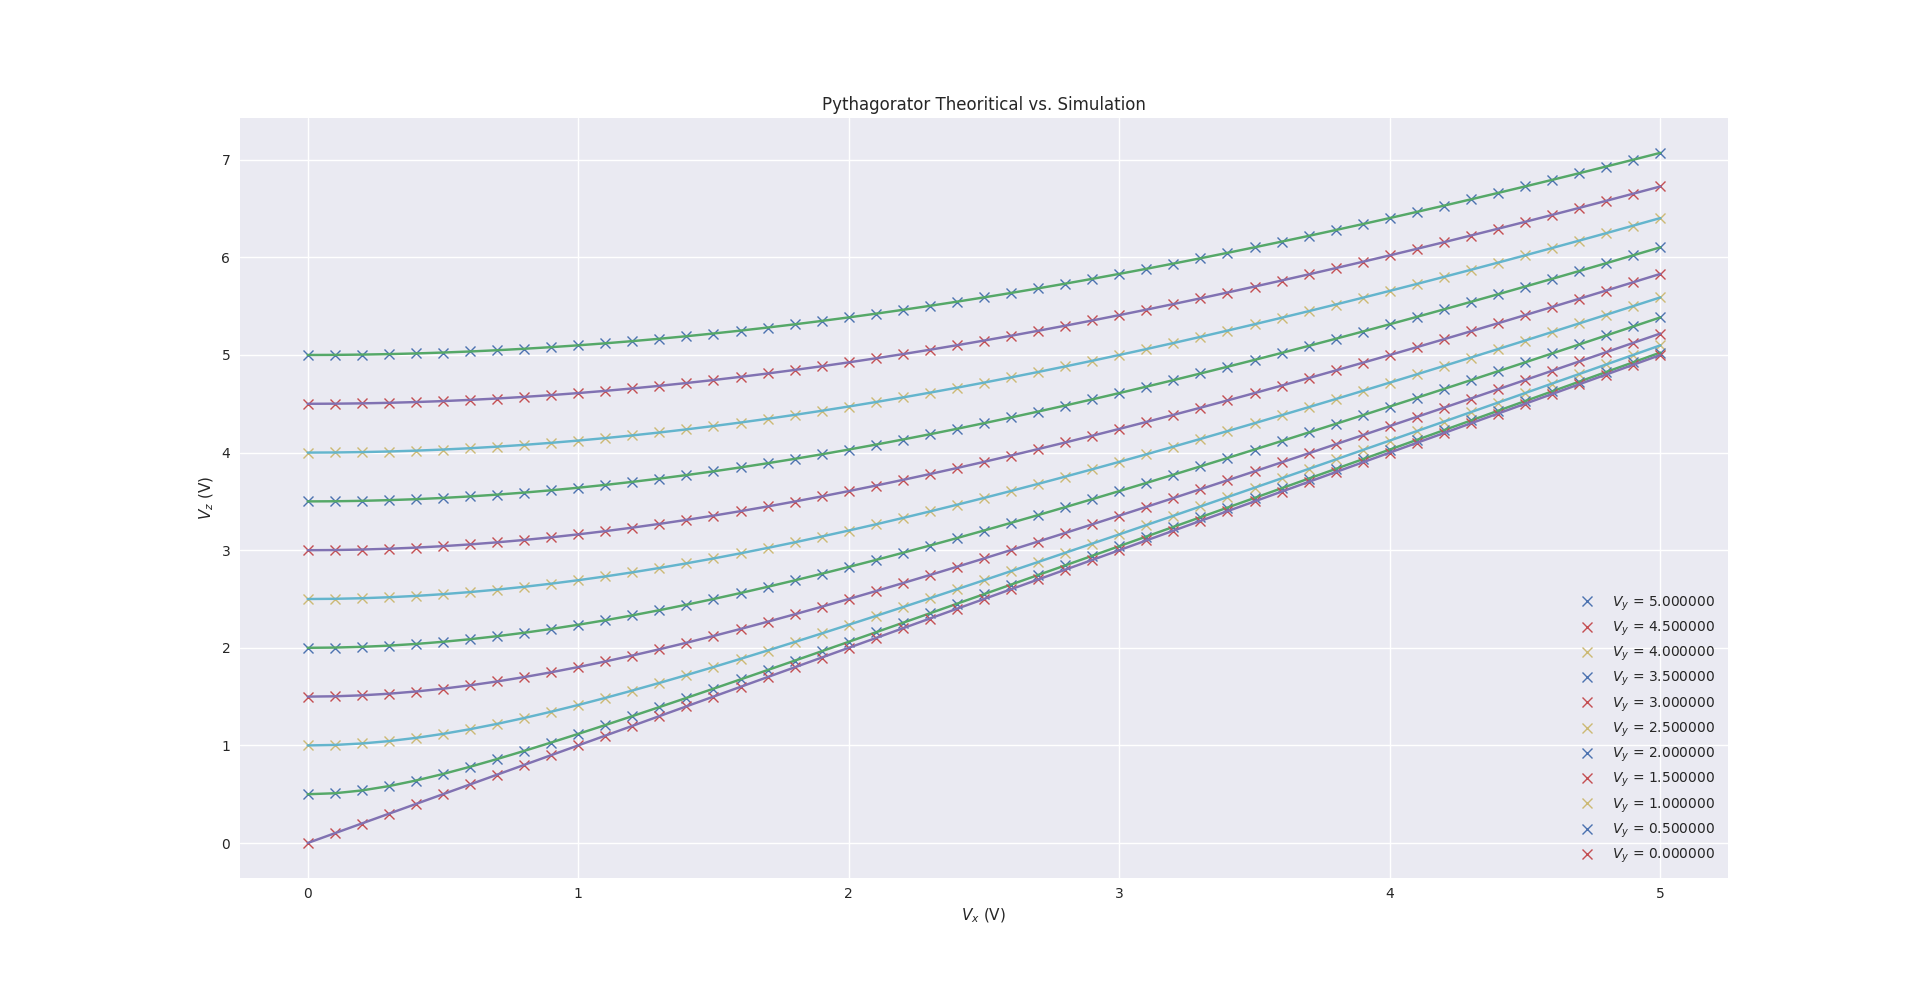
\includegraphics[width=\textwidth]{../figure1}
    \label{fig:1}
\end{figure}

As shown in \ref{fig:1}, the circuit does behave as I would expect.

\end{document}
